\documentclass[a4paper]{article}
\usepackage[pdftex]{hyperref}
\usepackage[latin1]{inputenc}
\usepackage[english]{babel}
\usepackage{a4wide}
\usepackage{amsmath}
\usepackage{amssymb}
\usepackage{algorithmic}
\usepackage{algorithm}
\usepackage{ifthen}
\usepackage{listings}
% move the asterisk at the right position
\lstset{basicstyle=\ttfamily,tabsize=4,literate={*}{${}^*{}$}1}
%\lstset{language=C,basicstyle=\ttfamily}
\usepackage{moreverb}
\usepackage{palatino}
\usepackage{multicol}
\usepackage{tabularx}
\usepackage{comment}
\usepackage{verbatim}
\usepackage{color}
\usepackage[utf8]{inputenc}
\usepackage{tabulary}
\usepackage{colortbl}

% Because of an error on line 41 I added this
\usepackage{graphicx}

% Used for drawing DFAs and NFAs
\usepackage{tikz}
\usetikzlibrary{automata, positioning}

%% pdflatex?
\newif\ifpdf
\ifx\pdfoutput\undefined
\pdffalse % we are not running PDFLaTeX
\else
\pdfoutput=1 % we are running PDFLaTeX
\pdftrue
\fi
%\ifpdf
%\usepackage[pdftex]{graphicx}
%\else
%\usepackage{graphicx}
%\fi
\ifpdf
\DeclareGraphicsExtensions{.pdf, .jpg}
\else
\DeclareGraphicsExtensions{.eps, .jpg}
\fi

\parindent=0cm
\parskip=0cm

\setlength{\columnseprule}{0.4pt}
\addtolength{\columnsep}{2pt}

\addtolength{\textheight}{5.5cm}
\addtolength{\topmargin}{-26mm}
\pagestyle{empty}

%%
%% Sheet setup
%% 
\newcommand{\coursename}{Formal Languages and Logic}
\newcommand{\courseno}{CO21-320211}
 
\newcommand{\sheettitle}{Homework}
\newcommand{\mytitle}{}
\newcommand{\mytoday}{October 30th, 2018}

% Current Assignment number
\newcounter{assignmentno}
\setcounter{assignmentno}{6}

% Current Problem number, should always start at 1
\newcounter{problemno}
\setcounter{problemno}{1}

%%
%% problem and bonus environment
%%
\newcounter{probcalc}
\newcommand{\exercise}[2]{
  \pagebreak[2]
  \setcounter{probcalc}{#2}
  ~\\
  {\large \textbf{Exercise \arabic{problemno}} \hspace{0.2cm}\textit{#1}} \refstepcounter{problemno}\vspace{2pt}\\}

\newcommand{\bonus}[2]{
  \pagebreak[2]
  \setcounter{probcalc}{#2}
  ~\\
  {\large \textbf{Bonus Problem \arabic{assignmentno}.\arabic{problemno}} \hspace{0.2cm}\textit{#1}} \refstepcounter{problemno}\vspace{2pt}\\}

%% some counters  
\newcommand{\assignment}{\arabic{assignmentno}}

%% solution  
\newcommand{\solution}{\pagebreak[2]{\bf Solution:}\\}

%% Hyperref Setup
\hypersetup{pdftitle={Homework \assignment},
  pdfsubject={\coursename},
  pdfauthor={},
  pdfcreator={},
  pdfkeywords={Formal Languages and Logic},
  %  pdfpagemode={FullScreen},
  %colorlinks=true,
  %bookmarks=true,
  %hyperindex=true,
  bookmarksopen=false,
  bookmarksnumbered=true,
  breaklinks=true,
  %urlcolor=darkblue
  urlbordercolor={0 0 0.7}
}

\begin{document}
\coursename \hfill Course: \courseno\\
Jacobs University Bremen \hfill \mytoday\\
Dragi Kamov and Dushan Terzikj\hfill
\vspace*{0.3cm}\\
\begin{center}
{\Large \sheettitle{} \assignment\\}
\end{center}

\exercise{}{0}
\solution
In order to build the PDA specified in the problem set, we need to differentiate three different state sets. Since $n,m,k\ge 1$, we need to transition to a state after reading the first character (\textbf{which should be 0 and no other}). Let us denote the disjoint state sets $S_0, S_1, and S_2$. After reading a character 0 we go to the state set $S_0$. State set $S_1$ can be reached when reading 1, only from state sets $S_0$ and $S_1$. When we read 2 we go to state set $S_2$ which is only reachable from state sets $S_1$ and $S_2$. Accepting states are in state set $S_2$. Since PDA has a stack, we insert 0 in the stack everytime we read one and pop a 0 whenever we read 1. In order to check $n\ne m$ one of the following has to happen:
\begin{enumerate}
    \item The PDA starts reading 1, but the stack has no more 0's. This means that $n\ne m$, therefore we can resume reading 1's or 2's. 
    \item The PDA starts reading 2's, but there are still 0's in the stack. This also means $n\ne m$ and we can continue reading 2's.
    \item It reads the first 2 exactly after the last 0 has been popped from the stack. This means $n=m$ and this word should not be accepted.
\end{enumerate}
Let us define a PDA $A(Q,\Sigma, \Gamma, \delta, q_0, Z_0, F):$
\begin{itemize}
    \item $Q=\{q_0, q_1, q_2, q_3\}$
    \item $\Sigma=\{0, 1\}$
    \item $\Gamma=\{Z_0, 0, 1\}$
    \item $\delta\leftarrow$\textbf{Transitions written below}
    \item $q_0\in Q$ is the starting state
    \item $Z_0\in \Gamma\leftarrow$ stack top symbol
    \item $F=\{q_3\}$
\end{itemize}
Here are the transitions:
\begin{enumerate}
    \item $\delta(q_0, 0, Z_0)=\{(q_0, 0Z_0)\}$
    \item $\delta(q_0, 0, 0)=\{(q_0, 00)\}$
    \item $\delta(q_0, 1, 0)=\{(q_1, \epsilon)\}$
    \item $\delta(q_1, 1, 0)=\{(q_1, \epsilon)\}$
    \item $\delta(q_1, 1, Z_0)=\{(q_2, Z_0)\}$
    \item $\delta(q_2, 1, Z_0)=\{(q_2, Z_0)\}$
    \item $\delta(q_2, 2, Z_0)=\{(q_3, Z_0)\}$
    \item $\delta(q_3, 2, *)=\{(q_3, *)\}\leftarrow$ \textbf{* means any symbol}
    \item $\delta(q_1, 2, 0)=\{(q_3, \epsilon)\}$
\end{enumerate}
\newpage
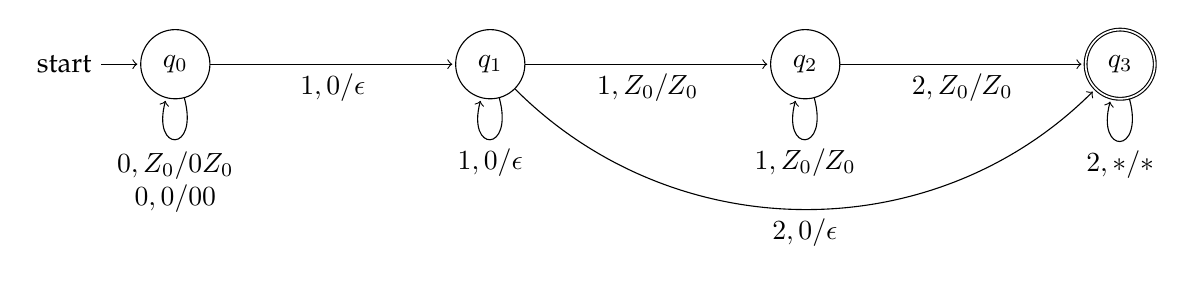
\begin{tikzpicture}[shorten >=1pt,node distance=4cm,on grid,auto] 
   \node[state,initial] (q_0)   {$ q_0 $}; 
   \node[state] (q_1) [right=of q_0] {$ q_1 $}; 
   \node[state] (q_2) [right=of q_1] {$ q_2 $}; 
   \node[state,accepting](q_3) [right=of q_2] {$ q_3 $};
    \path[->] 
    (q_0) edge [loop below] node {\begin{tabular}{c} $ 0,Z_0/0Z_0 $ \\ $ 0,0/00 $ \end{tabular}} ()
        edge node [swap] {$ 1,0/\epsilon $} (q_1)
    (q_1) edge [loop below] node {$ 1,0/\epsilon $} ()
        edge node [swap] {$ 1,Z_0/Z_0 $} (q_2)
        edge [bend left=-45] node [below] {$ 2,0/\epsilon$} (q_3)
    (q_2) edge [loop below] node {$ 1,Z_0/Z_0 $} ()
        edge node [swap] {$ 2,Z_0/Z_0 $} (q_3)
    (q_3) edge [loop below] node {$ 2,*/* $} ();
\end{tikzpicture}


\end{document}
